\documentclass[a4paper,11pt]{article}
\usepackage[margin=1in]{geometry}
\usepackage{array}
\usepackage{caption}
\usepackage{subcaption}

\usepackage[english]{babel}
\usepackage[utf8]{inputenc}
\usepackage{amsmath}
\usepackage{graphicx}
\graphicspath{ {images/} }
% \setlength{\textwidth}{390pt}
\setlength{\headheight}{34.5pt}
\usepackage{fancyhdr}
\pagestyle{fancy}

\usepackage{lipsum}

\newcommand{\exedout}{%
  \rule{0.8\textwidth}{0.5\textwidth}%
}


\makeatletter
\newcommand{\thickhline}{%
    \noalign {\ifnum 0=`}\fi \hrule height 1pt
    \futurelet \reserved@a \@xhline
}
\newcolumntype{"}{@{\hskip\tabcolsep\vrule width 1pt\hskip\tabcolsep}}
\makeatother


% \usepackage{showframe}

\title{Exploring the use of Big Data techniques for simulating Algorithmic Trading Strategies}

\author{Nishith Tirpankar, Jiten Thakkar\\
\texttt{tirpankar.n@gmail.com, jitenmt@gmail.com}}

\date{December 20, 2015}

\begin{document}
\maketitle
\thispagestyle{empty}
\begin{abstract}
In the world of information technology where huge amount of useful information is available and easily accessible, we investigate an approach to utilize this information in Algorithmic Trading. Algorithmic trading involves implementation of a strategy using computer programs to automatically buy and sell financial instruments to generate profit at a speed and frequency that is impossible for a human trader. High Frequency Trading (HFT) is one type of algorithmic trading characterized by high turnover and high order-to-trade ratios. There are different strategies that can be applied to HFT. We propose a framework to utilize information available in the form of news articles, which can be used in stock trading at high frequency. We use semantic values of news articles for different stocks to generate buy/sell signals at a high frequency. We demonstrate the performance of our framework by simulating stock trade based on generated buy/sell signals for a small period of time. 
\end{abstract}

\newpage
\tableofcontents
\thispagestyle{plain}
\setcounter{page}{1}
\newpage
\section{Introduction}
We live in a time and age where new information is generated at an unprecedented rate. More and more information is being published on the internet by individuals and corporations in different domains. People's reliance on this information is also increasing as access to quality information is becoming easy. In the field of stock markets, different news agencies and market research firms publish articles stating their opinion of the future of different stocks and different trends in the stock market. These articles are written after detailed research and analysis by market analysts. These articles are becoming a valuable source of information for independent investors who doesn't possess skills to analyze the stock market for their investment. As a result of this trend, they can influence the stock prices dramatically. For example, 
as observed by Leinwe-ber and Sisk (2011)\cite{leinwe}, a series of errors in 2008 lead to resurfacing of a 2002 article about United Airlines possibly filing for bankruptcy on Bloomberg - a leading financial services company, which then	set	off	a chain	reaction on	services that monitor Bloomberg. This resulted in the stock of United's parent company, UAL corporation, dropping 76 percent in six minutes. We think that stock related news articles can be utilized in HFT trading.
\par
Big trading institutions like hedge funds and mutual fund managers use sophisticated techniques and resources for performing HFT. That kind of resources are out of reach for an individual investor. It is impossible for an individual person to go through all the literature that is available and perform trading based on that. We propose a HFT platform which uses Big Data techniques to infer useful information from high volume of stock related news articles at high rate and frequency. This platform will automate the process of analyzing the news articles and it can be modified and tuned according to the user's needs.
\section{Related Work}
There are many attempts to use information available in electronic form to predict market trends. Leinwe-ber and Sisk (2011)\cite{leinwe} studied the effect of news in the past and the time needed to process the news in event-driven trading. Lee et al.\cite{lee} demonstrates a news monitoring and stock prediction system which uses 8k articles published by publicly listed companies in USA. Since it depends on 8K articles, it is limited to companies listed in USA. Our approach can be applied in any part of the world where there is stock related information available in electronic form.

\section{Theory}
HFT is a specialised form of algorithmic trading characterized by high turnover and high order-to-trade ratios. The strategies used in HFT need to be tested on historical data in order to ensure sound behaviour. We wish to test various strategies including some of our own on historical data and compare their results. An example of such a strategy is:
\par“Buy when the 50 day moving average of of a stock exceeds its 200 day average. Sell the stock if available if its 50 day moving average goes below its 200 day moving average.”
\par Verification of a trading strategy requires testing on a large amount of historical data. We will be verifying our strategy on historical data that we collected over the period of 10 days. HFT strategies can be divided in two categories:
\begin{itemize}
\item \textbf{Fundamental Analysis-}  This includes studying everything from the overall economy and industry conditions to the financial condition and management of companies.
\item \textbf{Technical analysis-}  This includes evaluation of securities by means of studying statistics generated by market activity, such as past prices and volume.
\end{itemize}
Our platform performs predictive analysis based on technical stock data. In this extension we look at financial news articles released online by various publishing firms to enhance the predictions. For this task we use 3 different sentiment analysis approaches(described in section \ref{Method}) using the ”textblob”\cite{textblob}, which is a sentiment analysis library in python. The task of sentiment analysis is complicated and coming up with our own technique is something we have scoped out of this project. Sentiment analysis of a sentence or text, quantifies the attitude of the author towards the general subject of the text. For example the sentence ”Among tech stocks Apple is a favorite” has a positive attitude. Hence, it will have a positive sentiment score. The sentiment score is a value between -1.0 and 1.0. A -1 signifies a negative sentiment while a +1 signifies a highly positive sentiment. After doing sentiment analysis of articles, the platform generates buy/sell signals at high frequency. These signals can are applied to HFT.
\section{Method} \label{Method}
In this section, we describe analysis techniques used in our platform in detail. We collect news articles related to a particular stock at a frequency of 15 minutes for all the stocks. This frequency can be changes later on by the user. We have used 15 minutes frequency in our results in Section \ref{result}. Section \ref{approaches} explains different sentiment analysis approaches used in the platform for these articles. The output of this sentiment analysis is used to generate buy/sell signals. The procedure to generate buy/sell signals is described in section \ref{signal generation}.

\subsection{Sentiment Analysis Approaches} \label{approaches}
We calculate sentiment values of articles according to following three approaches:
\begin{itemize}

\item \textbf{Article Level Sentiment-} In this approach, we calculate sentiment value for the whole article and take an average over all sentiment values of the articles in a particular interval. We only consider news articles which are related to the stock. We can represent Article Level Sentiment ($S_{als}$) as
\begin{equation}
S_{als} =  \big( 1/n \big)  \sum_{i=1}^n S_{i}
\end{equation}
where $S_{als}$ is Article Level Sentiment Value, $n$ is number of articles and $S_{i}$ is sentiment value for article $i$.

\item \textbf{Subjective Article Level Sentiment-} In this approach, we filter out objective sentence and calculate sentiment of the remaining text containing subjective sentences. Textblob library provides subjectivity for every sentence. We filter out sentences with subjectivity value less than or equal to zero. According to Pang et al \cite{pang} removing objective sentences from a document before classifying its polarity helped improve performance. Here, we only consider news articles which are related to the stock.

\item \textbf{Sentence Level Sentiment-} This approach does co-reference integration of the articles. In this approach, we use all the articles collected for all the stocks in a particular time interval. We also maintain a list of related key words like name of the company, stock symbol etc. for all the stocks. In order to calculate sentiment for a stock, we go through all the articles and consider only sentences containing key word for this particular stock. We calculate sentiment value of those sentences and take an average which represents sentiment value of the article for the stock. After calculating individual sentiment of all the articles for stock in consideration, we take an average over all the articles' sentiment values. We can represent Sentence Level Sentiment ($S_{sls}$) as
\begin{equation}
S_{sals} =  \big( 1/n \big)  \sum_{i=1}^n  \big( 1/q \big) \sum_{j=1}^q S_j^i
\end{equation}
where $S_sals$ is Sentence Level Sentiment for a stock, $n$ is the number of articles, $q$ is the number of sentences containing keyword related to stock in article $i$, $S_j^i$ is the sentiment value of sentence $j$ in article $i$.
\end{itemize}

\begin{figure}
\begin{subfigure}{.5\textwidth}
  \centering
  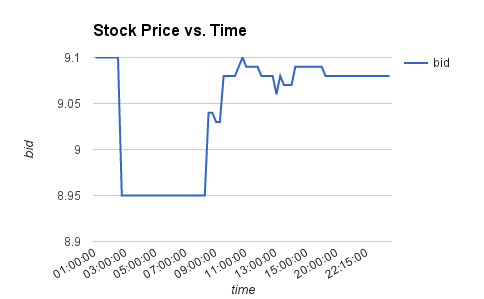
\includegraphics[width=.8\linewidth]{Stock_Price.png}
  \caption{Stock price for Apple Inc}
  \label{fig:sfig1}
\end{subfigure}%
\begin{subfigure}{.5\textwidth}
  \centering
  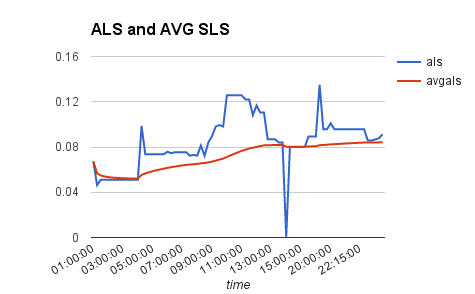
\includegraphics[width=.8\linewidth]{ALS.png}
  \caption{$S_{als}$ and $S_{avg}$ values}
  \label{fig:sfig2}
\end{subfigure}
\begin{subfigure}{.5\textwidth}
  \centering
  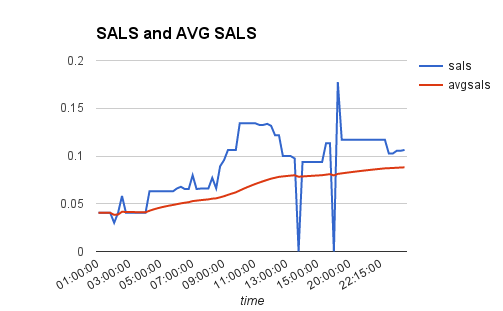
\includegraphics[width=.8\linewidth]{SALS.png}
  \caption{$S_{sals}$ and $S_{avg}$ values}
  \label{fig:sfig3}
\end{subfigure}%
\begin{subfigure}{.5\textwidth}
  \centering
  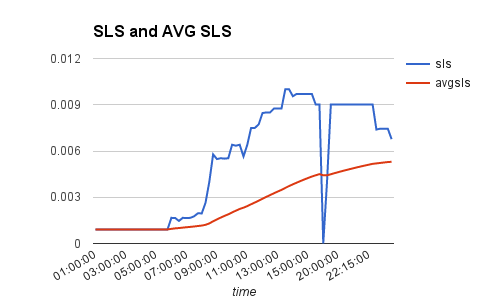
\includegraphics[width=.8\linewidth]{SLS.png}
  \caption{$S_{sls}$ and $S_{avg}$ values}
  \label{fig:sfig4}
\end{subfigure}
\caption{Stock prices and different sentiment values on 2015-11-24 for Apple Inc.}
\label{fig:fig}
\end{figure}

\subsection{Signal Generation} \label{signal generation}
In order to generate buy/sell signal using any sentiment analysis approach described above, we take and average of all the sentiment values of the stock over all the intervals before current interval($S_{avg}$) and compare that average value to the current sentiment value($S_{curr}$). Here, we generate buy/sell signals based on the logic - buy low and sell high. In order to make profit, we need to buy stocks at lower price and sell at higher price. So, if $S_{curr} > S_{avg}$, a \textbf{buy} signal is generated because according semantic values, it is likely that the stock value is going to increase compared to current value. If $S_{curr} < S_{avg}$, a \textbf{sell} signal is generated because according semantic values, it is likely that the stock value is going to decrease compared to current value.
\section{Data Collection}
This section describes data collection process that we used for out simulation. In out simulation we collect new articles and stock values for stocks in consideration. The stock values are collected to simulate stock trading. We use Yahoo! finance API for fetching this data in real time. For new articles, we use Yahoo! finance company news RSS feed \cite{news}. Using this API, we can fetch articles only related a particular stock. Since it is offered from Yahoo!, we can rely on the quality of the articles. This RSS feed contains only URL link of the article. Actual article is fetched at the time of processing. For stock prices, we use Yahoo! finance RSS feed which provides live stock values for stocks. We fetched news articles and stock value data every 15 minutes for some 3000 stocks for 10 days. Since there is a limit of 1000 Requests/Unique IP address/Day on Yahoo! API, as a work around, we deployed our data collection scripts in 10 different CADE computers as cron jobs and divided stocks among these 10 machines. Different CADE machines have different IP addresses. Everyday almost 4GB of data was being collected which contained news feed articles and stock prices. The number of unique articles was 68000 on average.
\par While processing news articles, we fetch the HTML pages. This HTML page contains unnecessary HTML tags and advertisement data. We use "newspaper" python package\cite{newspaper} for sanitizing the HTML page and extracting only article text. This text is used for sentiment analysis.
\section{Results} \label{result}
In order to measure the performance of our trading platform, we simulate stock trading based on buy/sell signals generated by the platform. We assume that we have unlimited amount of money and we can buy as many stocks as we want. We go through all the 15 minute intervals one by one and apply the following strategy for every semantic analysis approach for every stock:
\begin{itemize}
\item If platform generates buy signal then buy stocks worth \$1000
\item If platform generates sell signal then sell stocks worth \$1000
\end{itemize}
At the end of the simulation period, we sell all the stocks for the last known price of the stock and calculate profit/loss per stock. Since there were some technical issues in the data collection script, even if we collected data for 10 days only 4 days worth of data was useful. We show the results of this approach for 10 stocks for 4 days of data.
\begin{table}[]
\centering
\label{mylabel}
\begin{tabular}{|l||l|l|l|}
\hline
Stock Symbol & ALS & SLS & SALS \\\thickhline
AAWW & 6529.56 & 2814.68 & 5454.0 \\\hline
AA & 2356.83 & 1594.4 & 2257.24 \\\hline
AAMC & 2155.4 & -3256.1 & -2900.28 \\\hline
AAT & 30.23 & 8.25 & -2034.0 \\\hline
AAL & -105.61 & 144.88 & -89.33 \\\hline
AAPL & -68.95 & -135.52 & -127.28 \\\hline
AAN & -794.32 & 1998.68 & -2079.13 \\\hline
AAON & -311.2 & 14.4 & -48102.7 \\\hline
AAP & -545.04 & -714.3 & -454.98 \\\hline
AAOI & -119.73 & 4306.57 & 150.27 \\\hline
Total & 9127.16 & 6775.94 & -47926.19 \\\hline
\end{tabular}
\caption{Profit/Loss for different approaches (values in \$) }
\end{table}
The total profit and loss amounts for all the stocks used in simulation are shown in Table 1.
\section{Discussion and Future Work}
As we can see from the results Article Level Sentiment Analysis(ALS) and Sentence Level Sentiment Analysis(SLS) approaches are proving to be profitable where as Subjective Article Level Sentiment Analysis(SALS) approach is resulting in loss. As we can see from the results, considering only subjective sentences for sentiment analysis doesn't result in better sentiment indication. Although since we sell all the stock at the end of the simulation, regardless of the sentiment value, it is possible that we would have made profit using this approach had we sold the stocks in the future when there is a sell signal. As we can see in \ref{my-label}, for SALS approach, symbol AAON alone is responsible for loss of \$48102.7. If we don't consider that one stock in our final calculation, then SALS too shows profit of \$176.51.
\par We demonstrated that using our platform we can predict sentiment of the stock price values and based on that we can define a profitable strategy. This indicates  that  text  carries  predictive  power  for  stock  price movement.
\par In future, we plan to incorporate page rank of the news article page to calculate weighted average value of the sentiment analysis. As an additional feature, user should be able to add or remove his/her choice of news source to the platform.
\begin{thebibliography}{9}
\bibitem{leinwe}
\texttt{http://ssrn.com/abstract=1952914}
\bibitem{lee} 
Lee, Heeyoung, et al. "On the importance of text analysis for stock price prediction." Unpublished working paper \\\texttt{http://www.stanford.edu/\~{}jurafsky/pubs/lrec2014\_stocks.pdf} (2014).
\bibitem{textblob}
\texttt{https://textblob.readthedocs.org/en/dev/}
\bibitem{pang}
Pang, Bo; Lee, Lillian (2004). "A Sentimental Education: Sentiment Analysis Using Subjectivity Summarization Based on Minimum Cuts". Proceedings of the Association for Computational Linguistics (ACL). pp. 271–278.
\bibitem{news}
\texttt{https://developer.yahoo.com/finance/company.html}
\bibitem{finance}
\texttt{http://finance.yahoo.com/news/rssindex/}
\bibitem{newspaper}
\texttt{https://pypi.python.org/pypi/newspaper}
\end{thebibliography}

\end{document}